\section{Programming: K-Means Analysis}
In this assignment, we will implement the K-means algorithm and perform it on a breast cancer data set. Please follow the attached Python notebook to write and plot the functions.
\subsection{Part 1: K-means iteration function}
Write the K-means iteration function as is described in the notebook. Each iteration takes the data and current centroid values for each class as parameters, and returns both updated centroid values along with a list of labels telling which class each datapoint belongs to.
\begin{enumerate}
    \item  Fill in the table below by reporting the resulting cluster labels and resulting centroids from running the iteration function on the given parameters.
            \begin{center}
            \begin{tabular}{|c|c|c|c|}
                \hline
                \textbf{X} & \textbf{Initial Centroids} & \textbf{Resulting Cluster Labels} & \textbf{Resulting Centroids}  \\
                 \hline
                [[1], [2], [10], [12]]  & [1, 2] & \verb|[0, 1, 1, 1]|& \verb|[[1.0], [8.0]]|  \\ \hline
                [[1], [2], [10], [12]]  & [1, 8] & \verb|[0, 0, 1, 1]| & \verb|[[1.5], [11.0]]| \\ \hline
               [[1], [2], [10], [12]]  & [2, 2] & \verb|[0, 0, 0, 0]| & \verb|[[6.25], [2.0]]|  \\ \hline
                [[0,5,0],[0,5,0],[0,4,3],[0,3,4]] & [[2.5,0,0],[-2.5,0,0]] & \verb|[0, 0, 0, 0]| & [[0.0, 4.25, 1.75], [-2.5, 0.0, 0.0]]  \\ \hline
                
            \end{tabular}
            \end{center}
        
    \item 
    If an iteration of the k-means algorithm returns less than K classes, what might that indicate about the data?
	\newline
	\newline
	This might indicate that $K$ classes is too many, and that fewer classes would suffice.

\end{enumerate}


\subsection{Part 2: Putting the algorithm together}
Now write the whole K-means function using your iteration function, as is described in the notebook. The function takes in the data set with the number of classes and returns the final centroid values, the final list of labels telling which class each data point belongs to, and the number of K-means iterations.
\begin{enumerate}
    \item Put your 3 sanity-check graphs here.
\begin{figure}[H]
    	\centering
    	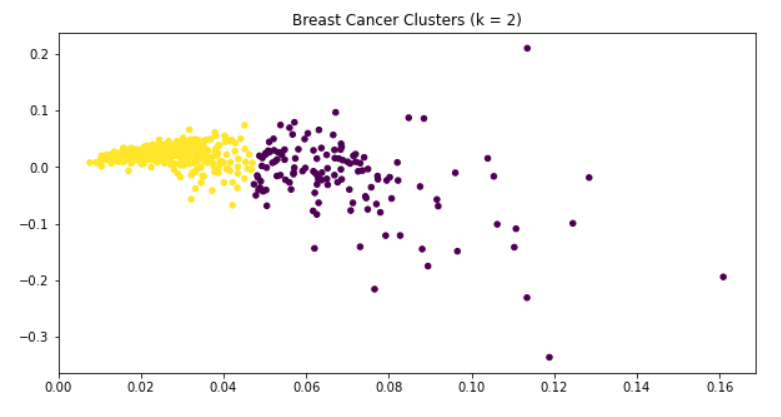
\includegraphics[width=.7\textwidth]{templates/k2}
    	\label{fig:my_label}
    \end{figure}
\begin{figure}[H]
    	\centering
    	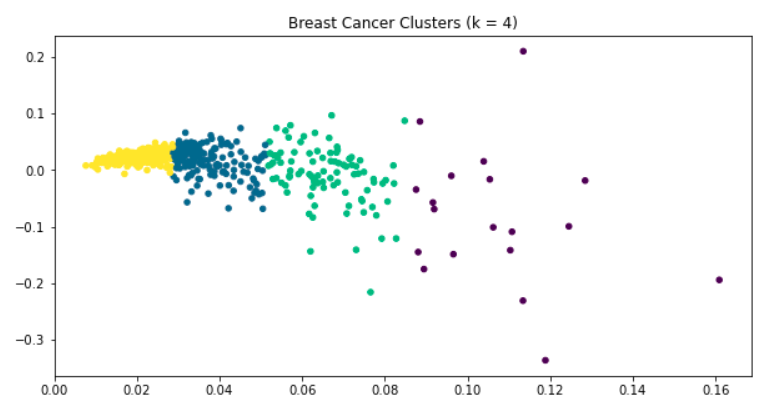
\includegraphics[width=.7\textwidth]{templates/k4}
    	\label{fig:my_label}
    \end{figure}
\begin{figure}[H]
    	\centering
    	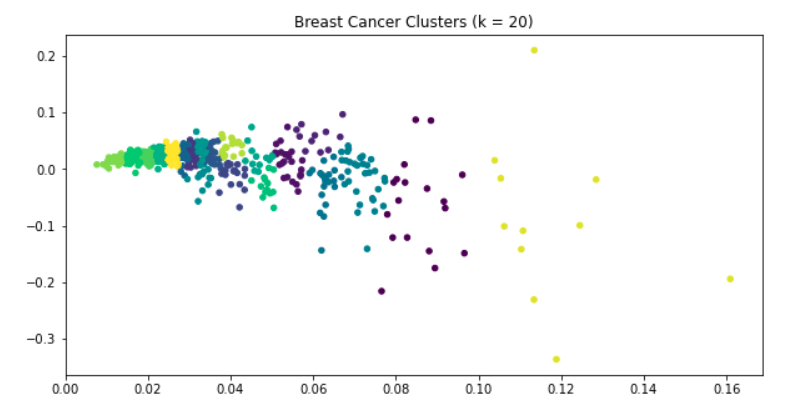
\includegraphics[width=.7\textwidth]{templates/k20}
    	\label{fig:my_label}
    \end{figure}
    
    \item Write down how many iterations it took for your k-means to converge for each of the sanity-check graphs. How does this number compare with what you expected it to be? How does the number of iterations seem to vary proportional to k?
    \begin{itemize}
\item $k = 2$ took 8 iterations.
\item $k = 4$ took 22 iterations.
\item $k = 20$ took 19 iterations.
    \end{itemize}

        The number of iterations seems to be positively correlated with $k$ for $k < 10$ but this relationship seems to break down for large $k$ such as $k = 20$. This indicates that convergence speeds up for large $k$ because the number of points in each class decreases as $k$ increases.
\end{enumerate}
\subsection{Part 3: Choosing the value of K}
Write the test$\_$cluster$\_$size function using your k-means function, as is described in the notebook. The function takes in the data set with the number of classes and returns a list of scores where each score is the distortion for that value of k.
\begin{enumerate}
    \item Using the breast cancer data set, record your labeled plots for distortion, min-max scaled distortion, and log scaled distortion here
    \newline
    \begin{figure}[H]
        	\centering
        	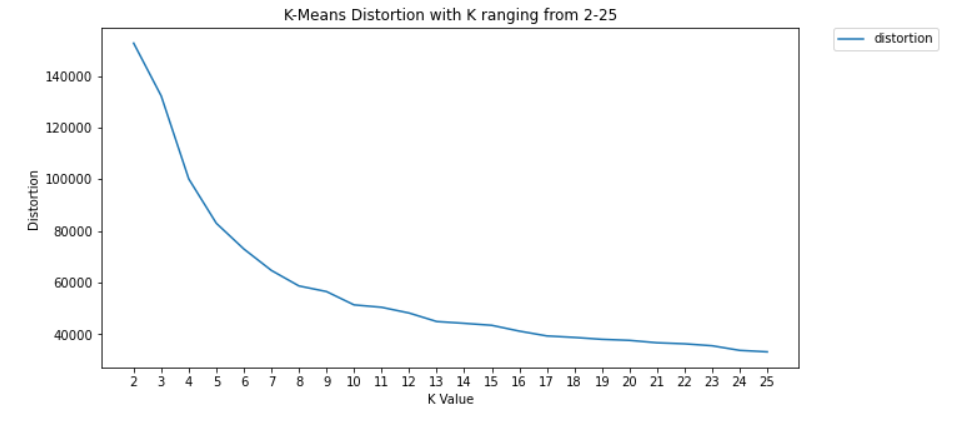
\includegraphics[width=.7\textwidth]{templates/distortion}
        	\label{fig:my_label}
        \end{figure}
\begin{figure}[H]
    	\centering
    	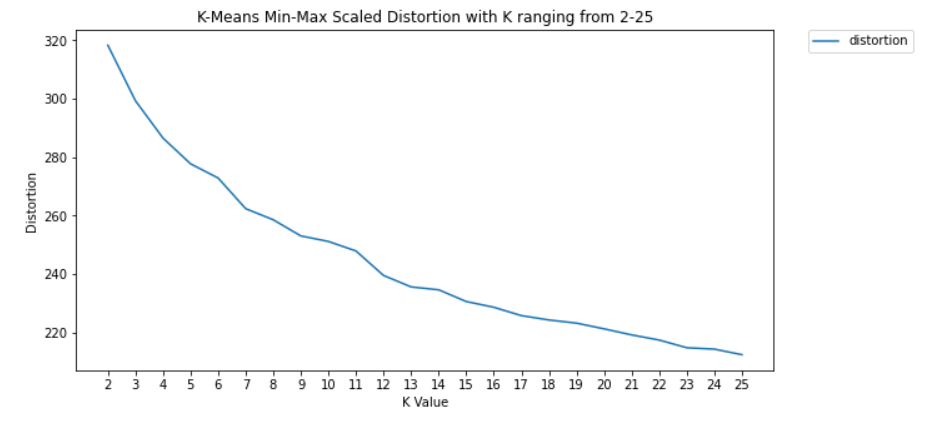
\includegraphics[width=.7\textwidth]{templates/scaled_distortion}
    	\label{fig:my_label}
    \end{figure}
\begin{figure}[H]
    	\centering
    	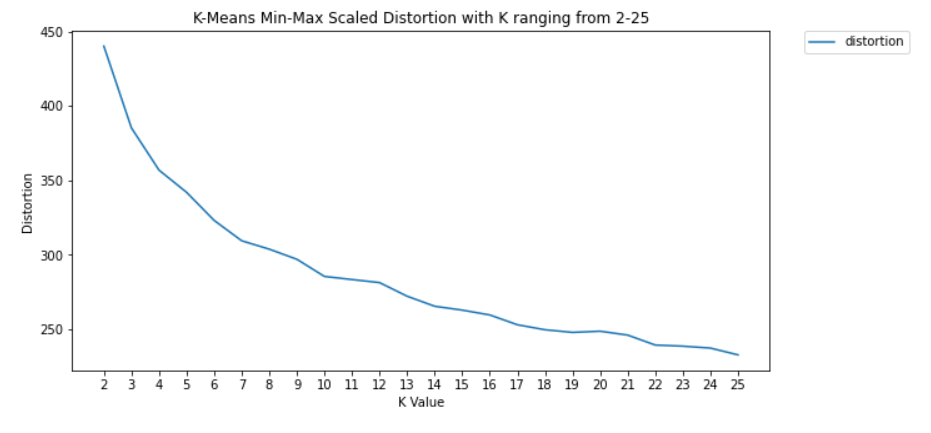
\includegraphics[width=.7\textwidth]{templates/minmax_distortion}
    	\label{fig:my_label}
    \end{figure}            
    \item Why can't we hold out some of the data in a validation set, and choose the value of k which minimizes a cross-validation error like we have in the past for algorithms like linear regression?
    \newline
    \newline
    We were able to hold out some of the data in a validation set when performing linear regression because it is a supervised learning problem. In this case, we are not able to do this because this is an unsupervised learning problem where there is no validation error we are trying to minimize.
\end{enumerate}
